\documentclass{beamer}
\usetheme{metropolis}
\usepackage{graphicx}
\usepackage{subfig}
\usepackage{tcolorbox}
\usepackage{mathtools}
\title{Algebra-Based Physics: Electricity, Magnetism, and Modern Physics (PHYS135B): Unit 4}
\author{Jordan Hanson}
\institute{Whittier College Department of Physics and Astronomy}

\begin{document}
\maketitle

\section{Summary}

\begin{frame}{Summary}
\begin{enumerate}
\item Magnetic induction - \textbf{Chapters 23.1 - 23.5, 23.7, 23.9}
\begin{itemize}
\item Induced EMF and magnetic flux
\item Faraday's Law
\item Motional EMF, generators, and transformers
\end{itemize}
\item AC circuits - \textbf{Chapters 23.9 - 23.12}
\begin{itemize}
\item Inductors
\item RL circuits
\item RLC circuits
\end{itemize}
\end{enumerate}
\end{frame}

\section{Magnetic induction}

\begin{frame}{Magnetic induction}
\small
\textbf{\alert{First set of observations:}} a \textit{moving} magnet can induce an emf in a coil of wire.  The induced current polarity depends on (a) magnet polarity and (b) direction of magnet velocity.  The induced current magnitude 
\begin{figure}
\centering
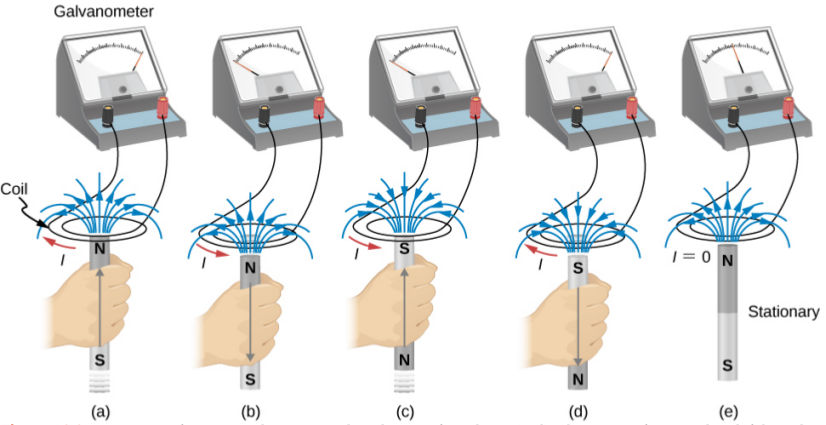
\includegraphics[width=0.8\textwidth]{figures/farad.png}
\caption{\label{fig:farad1} Observations of magnetic induction.}
\end{figure}
\end{frame}

\begin{frame}{Magnetic induction}
\small
\textbf{\alert{Second set of observations:}} a \textit{changing} current in a loop can induce an emf in another loop.  The induced current polarity depends on (a) inducing current polarity and (b) whether the inducing current is increasing or descreasing.
\begin{figure}
\centering
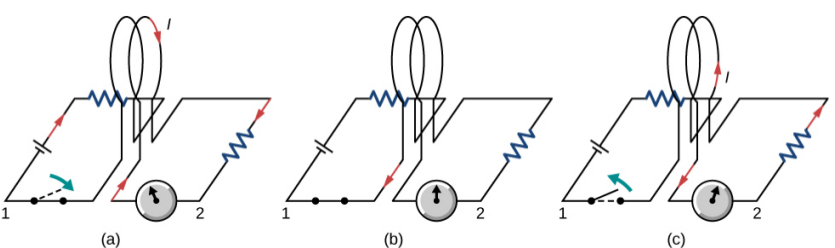
\includegraphics[width=0.8\textwidth]{figures/farad2.png}
\caption{\label{fig:farad2} Observations of magnetic induction.}
\end{figure}
\end{frame}

\begin{frame}{Magnetic induction}
\small
\textbf{\alert{Third observation:}} a \textit{changing} loop area in a magnetic field induces an emf, and current.  The induced current polarity depends on whether the loop area is (a) increasing or (b) descreasing.  The current magnitude depends on how quickly the area is changing.
\begin{figure}
\centering
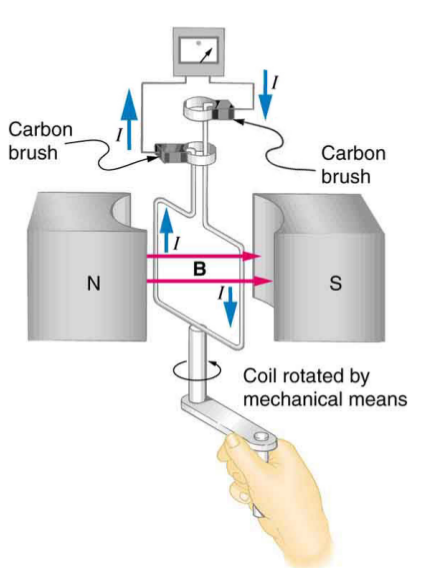
\includegraphics[width=0.3\textwidth]{figures/motorz.png}
\caption{\label{fig:motorz} Observations of magnetic induction.}
\end{figure}
\end{frame}

\begin{frame}{Magnetic induction}
Video summary of magnetic induction: \\
\url{https://youtu.be/pQp6bmJPU_0}
\begin{itemize}
\item Magnet inducing current in loop of wire
\item Solenoids inducing current in adjacent solenoids
\item Magnetic flux
\item Faraday's Law
\item Lenz's Law
\end{itemize}
\end{frame}

\begin{frame}{Magnetic induction}
\small
\textbf{\alert{Magnetic flux}} is the dot-product of the area vector and the magnetic field through loops of wire with area $A$.
\begin{columns}[T]
\begin{column}{0.5\textwidth}
\begin{figure}
\centering
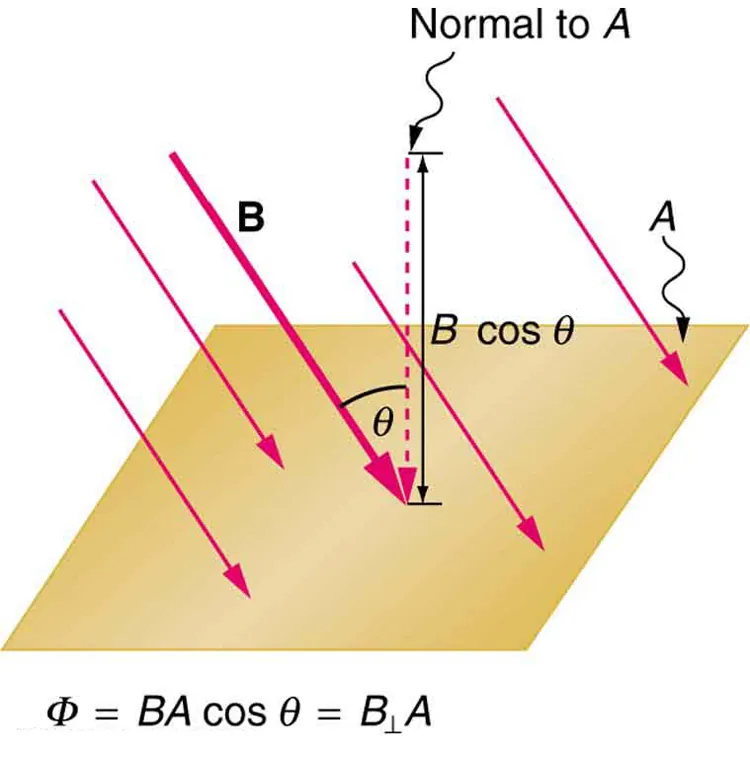
\includegraphics[width=0.95\textwidth]{figures/flux.png}
\caption{\label{fig:farad3} The \textbf{area vector} is \textit{normal} to the loop area.}
\end{figure}
\end{column}
\begin{column}{0.5\textwidth}
\vspace{0.5cm}
The \textbf{area vector} has a magnitude $A$, the area of the loop.  The direction of the area vector is \textit{normal} to the area of the loop.
\begin{equation}
\vec{A} = A \hat{n}
\end{equation}
The magnetic flux, $\Phi$, is therefore
\begin{equation}
\Phi = \vec{B} \cdot \vec{A}
\end{equation}
\end{column}
\end{columns}
\end{frame}

\section{Faraday's Law}

\begin{frame}{Faraday's Law}
\begin{tcolorbox}[colback=white,colframe=black!40!black,title=Faraday's Law]
\alert{Let the product of the magnetic field and the vector area be the magnetic flux: $\Phi = \vec{B} \cdot \vec{A}$.  The induced emf $\epsilon$ in $N$ turns of a conductor will be
\begin{equation}
\epsilon = - \frac{\Delta\Phi}{\Delta t}
\label{eq:farad}
\end{equation}
The induced current from $\epsilon$ will create a new B-field that opposes changes in $\Phi$.}
\end{tcolorbox}
\textit{The unit of magnetic flux is the Weber, or 1 Wb = 1 T m$^2$.}
\end{frame}

\begin{frame}{Faraday's Law}
\small
\begin{figure}
\centering
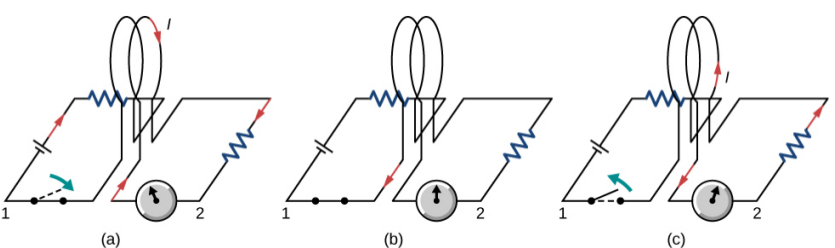
\includegraphics[width=0.7\textwidth]{figures/farad2.png}
\caption{\label{fig:loop1} A pickup coil system.}
\end{figure}
Suppose the switch in Fig. \ref{fig:loop1} (a) is closed, inducing a current $I$ in the right-hand loop.  The B-field directions at the centers of the left and right loops are
\begin{itemize}
\item A: Right and left, respectively
\item B: Light and right, respectively
\item C: Both to the right
\item D: Both to the left
\end{itemize}
\end{frame}

\begin{frame}{Faraday's Law}
\small
\begin{figure}
\centering
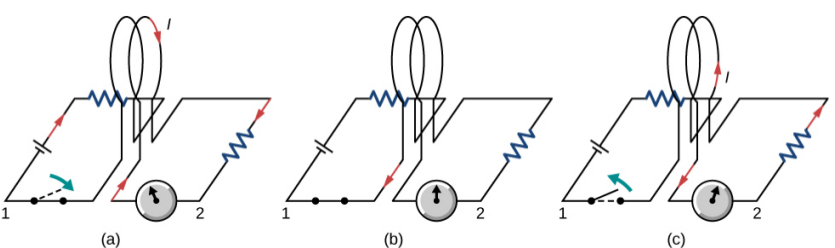
\includegraphics[width=0.7\textwidth]{figures/farad2.png}
\caption{\label{fig:loop2} A pickup coil system.}
\end{figure}
Suppose the switch in Fig. \ref{fig:loop1} (b) remains closed, and no induced current is observed.  This is because
\begin{itemize}
\item A: The magnetic flux is zero
\item B: The inducing current is zero
\item C: The magnetic flux is not changing
\item D: The loop area is zero
\end{itemize}
\end{frame}

\begin{frame}{Faraday's Law}
\small
\begin{figure}
\centering
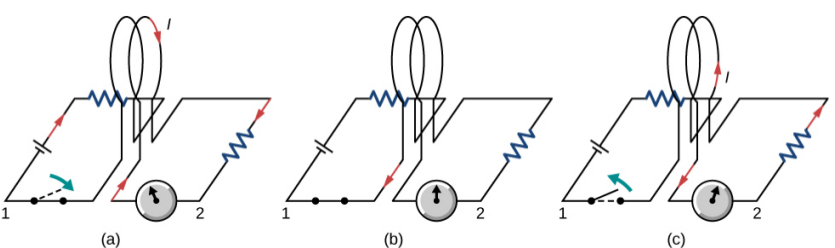
\includegraphics[width=0.7\textwidth]{figures/farad2.png}
\caption{\label{fig:loop3} A pickup coil system.}
\end{figure}
Suppose the switch in Fig. \ref{fig:loop1} (b) remains closed, and no induced current is observed.  This is because
\begin{itemize}
\item A: The magnetic flux is zero
\item B: The inducing current is zero
\item C: The magnetic flux is not changing
\item D: The loop area is zero
\end{itemize}
\end{frame}


\begin{frame}{Faraday's Law}
\small
\begin{figure}
\centering
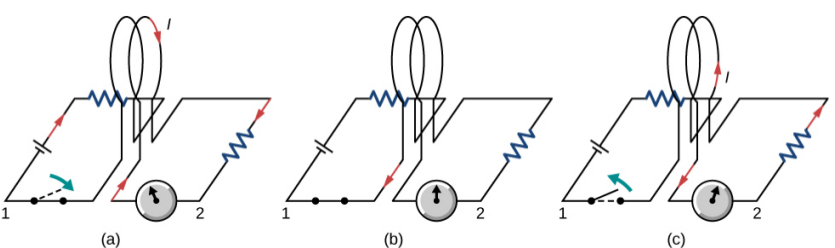
\includegraphics[width=0.7\textwidth]{figures/farad2.png}
\caption{\label{fig:loop4} A pickup coil system.}
\end{figure}
Suppose the switch in Fig. \ref{fig:loop1} (c) is opened.  The induced current in Fig. \ref{fig:loop1} is in the opposite direction of Fig. \ref{fig:loop1} (c) because
\begin{itemize}
\item A: The magnetic field from the right loop decreased
\item B: The magnetic field from the left loop increased
\item C: The magnetic field from the left loop is constant
\item D: The magnetic field from the left loop decreased
\end{itemize}
\end{frame}

\begin{frame}{Faraday's Law}
\small
\textbf{Group board problem:} \\ \vspace{0.5cm}
A magnetic field B passes orthogonally through a circular coil of radius $r = 0.05$ m and $N = 100$ turns.  The field magnitude decreases linearly according to
\begin{equation}
B(t) = B_0 - a t
\end{equation}
with $B_0 = 0.015$ T and $a = 0.01$ T s$^{-1}$.  (a) Calculate the magnitude of the emf induced in the coil at the times $t_0 = 0$, and $t_2 = 1.0$ second. (b) Determine the current in the coil if the resistance is 1 $\Omega$. \\ \vspace{0.5cm}
Sketch this system, and indicate both the direction of the instantaneous B-field, and the direction of current.
\end{frame}

\begin{frame}{Faraday's Law - PhET Activity}
\small
Brief simulation of Faraday's Law, and Lenz's Law: \\ \vspace{0.5cm}
\footnotesize
\url{https://phet.colorado.edu/en/simulations/faradays-law}
\small
\begin{enumerate}
\item Learn to control the position and orientation of the bar magnet.
\item Activate the voltmeter in parallel with the light bulb.
\item Use the coil with four loops of wire.
\item Produce the following results:
\begin{itemize}
\item A positve voltage from a moving bar magnet
\item A negative voltage from a moving bar magnet
\item A positive voltage from switching the bar magnet polarity
\item A negative voltage from switching the bar magnet polarity
\end{itemize}
\item Is your voltage positive or negative when you are increasing $\Phi$?  How do you \textit{decrease} $\Phi$?
\end{enumerate}
\end{frame}

\section{Motional EMF, Generators, and Transformers}

\begin{frame}{Motional EMF, Generators, and Transformers}
\small
\begin{figure}
\centering
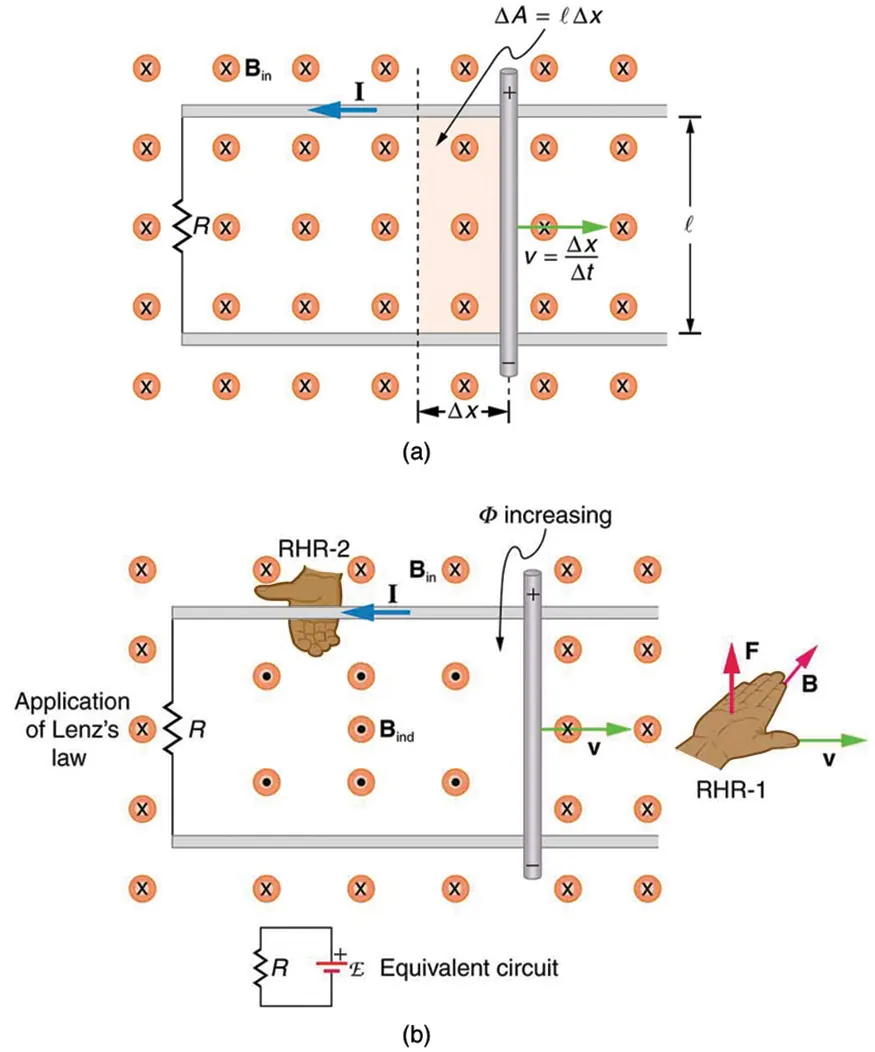
\includegraphics[width=0.44\textwidth,trim=4cm 20cm 4cm 0cm,clip=true]{figures/motion_emf.png}
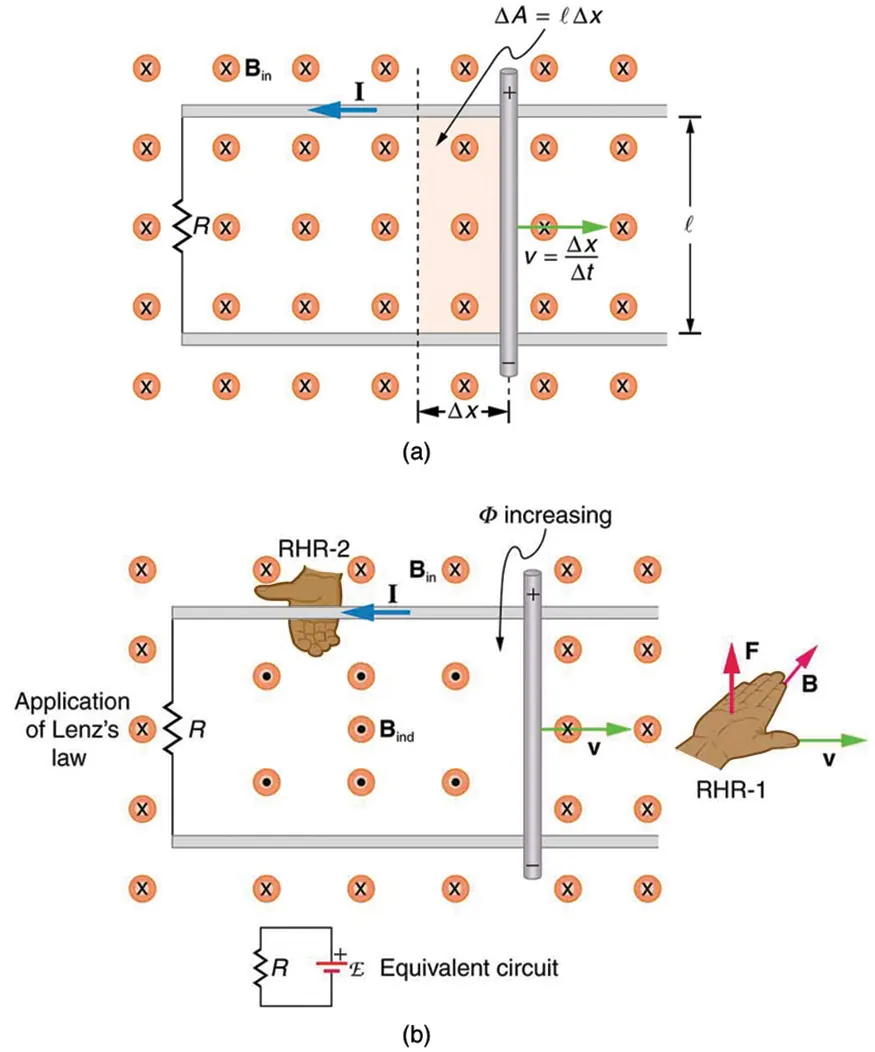
\includegraphics[width=0.54\textwidth,trim=0cm 0cm 0cm 18cm,clip=true]{figures/motion_emf.png}
\caption{\label{fig:motion_emf1} Motional emf in a loop with changing area.}
\end{figure}
\footnotesize
\textbf{\alert{Group board problems:}}
\begin{enumerate}
\item Show that \textit{power} is $P = \vec{F} \cdot \vec{v}$ when acceleration is constant.
\item Show that the emf is $\epsilon = B l v$, where $l$ is the length of the rod.
\item Show that power generated, $P = I^2 R = \epsilon/R$, is equal to power injected.
\end{enumerate}
\end{frame}

\begin{frame}{Motional EMF, Generators, and Transformers}
How do we use Faraday's Law to induce power in a generator?  Start with Faraday's Law:
\begin{equation}
\epsilon = - N\frac{\Delta \Phi}{\Delta t}
\end{equation}
The flux $\Phi$ depends on time:
\begin{equation}
\Phi = \vec{B} \cdot \vec{A}(t) = BA\cos(\theta(t))
\end{equation}
Let the \textit{angular velocity} be constant: $\theta = \omega t$.  Then we have
\begin{equation}
\Phi  = BA\cos(\omega t)
\end{equation}
Thus the emf (with $N$ loops) is (...calculus...)
\begin{equation}
\epsilon = N\omega BA \sin(\omega t) = \epsilon_0 \sin(\omega t)
\end{equation}
\end{frame}

\begin{frame}{Motional EMF, Generators, and Transformers}
\footnotesize
\begin{figure}
\centering
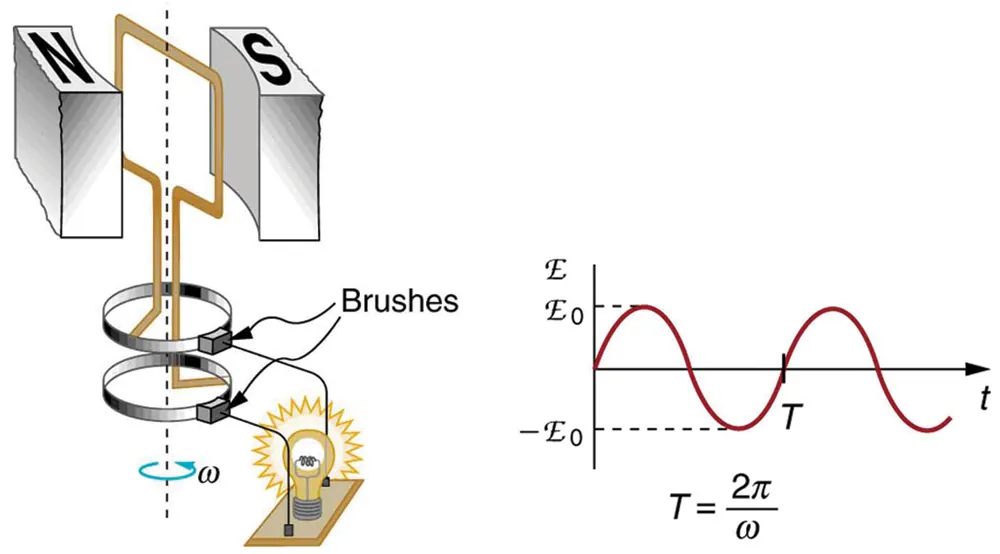
\includegraphics[width=0.65\textwidth]{figures/generator_1.png}
\caption{\label{fig:motion_emf2} (Left) The AC generator with brushes generates an AC voltage. (Right) This is a diagram of the AC voltage.}
\end{figure}
\begin{itemize}
\item Amplitude: $\epsilon_0$, the maximum value of the AC signal. Units: Volts.
\item Period: $T = 2\pi/\omega$, the time to complete one AC cycle.  Units: seconds.
\item Frequency: $f = 1/T$, the number of cycles per second.  Units: Hertz.
\end{itemize}
\end{frame}

\begin{frame}{Motional EMF, Generators, and Transformers}
\footnotesize
\begin{figure}
\centering
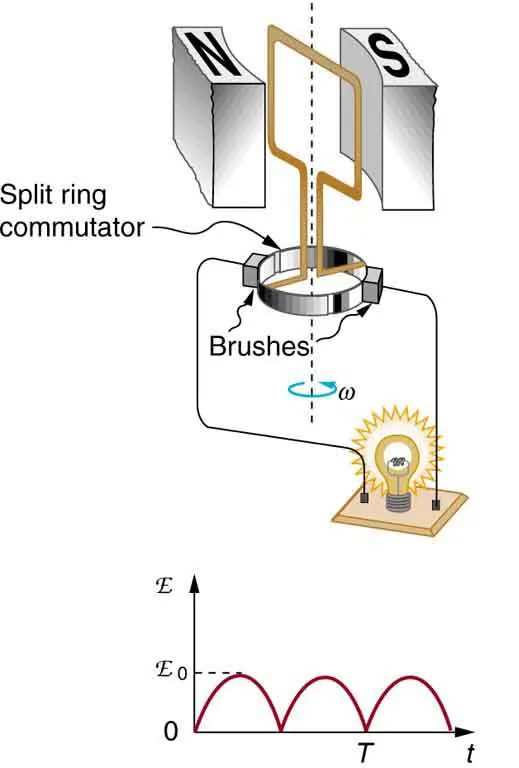
\includegraphics[width=0.35\textwidth,trim=0cm 8cm 0cm 0cm,clip=true]{figures/generator_2.png}
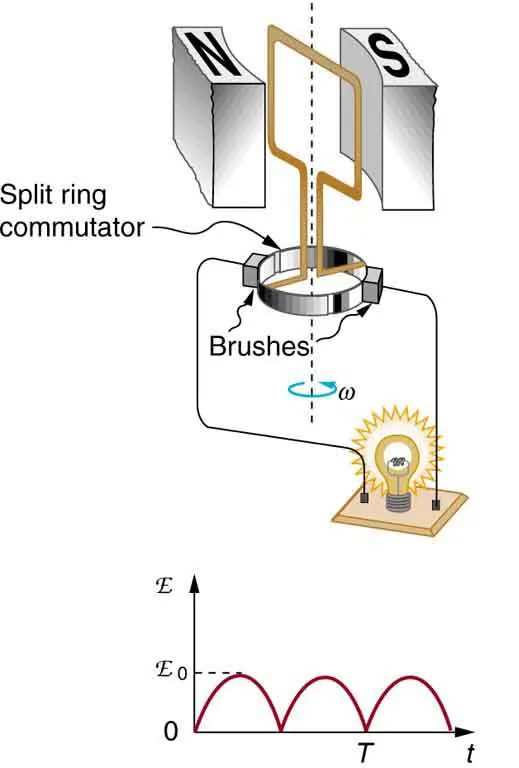
\includegraphics[width=0.5\textwidth,trim=0cm 0cm 0cm 20cm,clip=true]{figures/generator_2.png}
\caption{\label{fig:motion_emf3} (Left) The AC generator with brushes and \textit{commutator} generates pulsed DC. (Right) This is a diagram of the signal.}
\end{figure}
\begin{itemize}
\item Amplitude: $\epsilon_0$, the maximum value of the AC signal. Units: Volts.
\item Period: $T = 2\pi/\omega$, the time to complete one AC cycle.  Units: seconds.
\item Frequency: $f = 1/T$, the number of cycles per second.  Units: Hertz.
\end{itemize}
\end{frame}

\begin{frame}{Motional EMF, Generators, and Transformers}
Equation \ref{eq:gen} is a basic model for the emf from a generator.
\begin{equation}
\epsilon = N\omega BA \sin(\omega t) = \epsilon_0 \sin(\omega t) \label{eq:gen}
\end{equation}
Which of the following would increase the \textit{amplitude} of the emf?
\begin{itemize}
\item A: Turning the shaft more slowly
\item B: Turning the shaft more quickly
\item C: Decreasing the B-field
\item D: Increasing $N$
\end{itemize}
\end{frame}

\begin{frame}{Motional EMF, Generators, and Transformers}
Equation \ref{eq:gen2} is a basic model for the emf from a generator.
\begin{equation}
\epsilon = N\omega BA \sin(\omega t) = \epsilon_0 \sin(\omega t) \label{eq:gen2}
\end{equation}
Which of the following would increase the \textit{frequency} of the emf?
\begin{itemize}
\item A: Turning the shaft more slowly
\item B: Turning the shaft more quickly
\item C: Decreasing the B-field
\item D: Increasing $N$
\end{itemize}
\end{frame}

\begin{frame}{Motional EMF, Generators, and Transformers}
Equation \ref{eq:gen3} is a basic model for the emf from a generator.
\begin{equation}
\epsilon = N\omega BA \sin(\omega t) = \epsilon_0 \sin(\omega t) \label{eq:gen3}
\end{equation}
\textbf{Group exercise:} Suppose an AC generator rotates at 200 rpm, in a B-field with 0.1 T, and has 100 loops with radius 5 cm.  (a) What is the peak voltage this generator will produce? (b) If the generator powers a system with resistance of 1k$\Omega$, what will be the peak current?
\end{frame}

\section{PhET: Motional EMF, Generators, and Transformers}

\begin{frame}{PhET: AC Power generator}
\footnotesize
Link to the (CheerpJ) simulation: \\ \vspace{0.2cm}
\url{https://phet.colorado.edu/en/simulation/generator}
\begin{enumerate}
\item Set the water rate such that the meter reads 10 rotations per minute (rpm).
\item Choose the voltage meter under the pickup coil menu.
\item Under loops, choose 1 loop, and under area, leave it at 50\%.
\item Choose show field meter in the upper right, and place the tool in the loop center.
\item On the same graph, plot the average B-field and voltage versus time.  What is the period and amplitude of your signal?  Use the left y-axis for B-field units, and the right y-axis for voltage units.
\item Create the same graph for $N = 3$ loops.
\item Create the same graph for $N = 1$ loop, but for 20 rpm.
\end{enumerate}
\textit{Hint: you know the rpm of the magnet, so you know how much time corresponds to one rotation.}
\end{frame}

\begin{frame}{Motional EMF, Generators, and Transformers}
\small
\begin{figure}
\centering
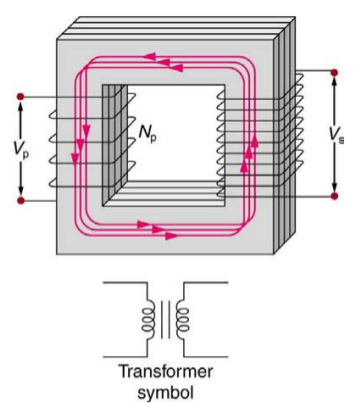
\includegraphics[width=0.45\textwidth,trim=0cm 5cm 0cm 0cm,clip=true]{figures/transformer.png}
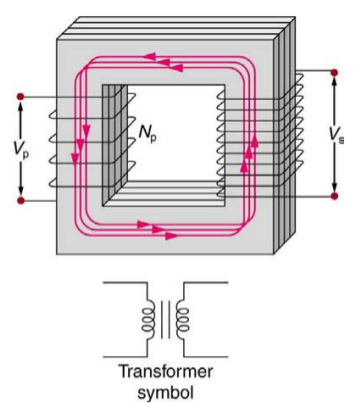
\includegraphics[width=0.25\textwidth,trim=3.0cm 0cm 4cm 10cm,clip=true]{figures/transformer.png}
\caption{\label{fig:trans1} A \textit{transformer} uses Faraday's law to change voltages in AC-generated systems.}
\end{figure}
The magnetizable core (gray) creates a loop in the B-field that passes through the left and right coils.  Use Faraday's law to show that
\begin{equation}
\frac{V_L}{V_R} = \frac{N_L}{N_R}
\end{equation}
\end{frame}

\begin{frame}{Motional EMF, Generators, and Transformers}
\begin{figure}
\centering
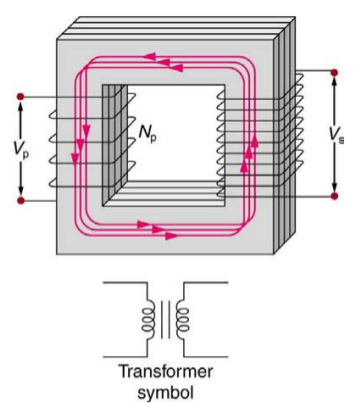
\includegraphics[width=0.35\textwidth,trim=0cm 5cm 0cm 0cm,clip=true]{figures/transformer.png}
\caption{\label{fig:trans2} The \textit{transformer} changes AC voltage levels.}
\end{figure}
Suppose the transformer in Fig. \ref{fig:trans2} has $N_L = 5$, $N_R = 100$, $V_L = 1$ kV (peak).  What is $V_R$ (peak), in kV?
\begin{itemize}
\item A: 20 kV
\item B: 5 kV
\item C: 0.05 kV
\item D: 0.05 V
\end{itemize}
\end{frame}

\begin{frame}{Motional EMF, Generators, and Transformers}
\begin{figure}
\centering
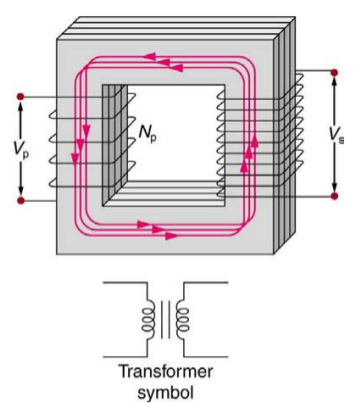
\includegraphics[width=0.35\textwidth,trim=0cm 5cm 0cm 0cm,clip=true]{figures/transformer.png}
\caption{\label{fig:trans3} The \textit{transformer} changes AC voltage levels.}
\end{figure}
\footnotesize
Suppose we need the transformer in Fig. \ref{fig:trans3} to produce $V_R = 120$ V, and $V_L = 12$ kV.  Which combination of coils will satisfy the requirement?
\begin{itemize}
\item A: $N_L = 3$, $N_R = 10$
\item B: $N_L = 10$, $N_R = 1000$
\item C: $N_L = 10$, $N_R = 100$
\item D: $N_L = 1000$, $N_R = 10$
\end{itemize}
\end{frame}

\begin{frame}{Motional EMF, Generators, and Transformers}
\footnotesize
\begin{figure}
\centering
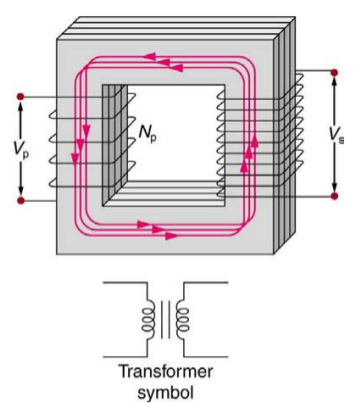
\includegraphics[width=0.25\textwidth,trim=0cm 5cm 0cm 0cm,clip=true]{figures/transformer.png}
\caption{\label{fig:trans4} \footnotesize The \textit{transformer} changes AC voltage levels.}
\end{figure}
If the $V_L \neq V_R$, how are energy and power conserved?
\begin{itemize}
\item A: The induced current is larger on the right.
\item B: The induced current is smaller on the right.
\item C: The induced current is conserved from left to right.
\item D: The induced emf is conserved from left to right.
\end{itemize}
\footnotesize
\textit{Demonstrate on board how power is conserved by (a) deriving the currents $I_L$ and $I_R$, then forming the powers $P_L$ and $P_R$.}
\end{frame}

\section{Inductors}

\begin{frame}{Inductors}
It turns out you can \textit{reverse} transformers, through symmetry.  Between the coils in the transformer in Fig. \ref{fig:trans4}, there is \textit{mutual inductance,} $M$:
\begin{align}
\epsilon_R &= -M \frac{\Delta I_L}{\Delta t} \\
\epsilon_L &= -M \frac{\Delta I_R}{\Delta t}
\end{align}
The \textbf{\alert{inductance}} accounts for everything except the current: the geometry, number of turns, and field strength.  Inductance is useful for systems with fixed geometry, where we often do not need to know $\Phi$. \\ \vspace{0.5cm}
\textbf{Derive} an expression that relates $M$ to $\Phi$, given the original version of Faraday's Law.
\end{frame}

\begin{frame}{Inductors}
Consider the case of \textbf{\alert{self-inductance}}, $L$, which accounts for the magnetic field created inside (for example) a solenoid when current is introduced.  New current creates a change in $\Phi$ within the solenoid, so Faraday's Law predicts a backwards emf opposing the change:
\begin{equation}
\boxed{
\epsilon = -L \frac{\Delta I}{\Delta t}}
\end{equation}
\footnotesize
The inductance unit is the \textit{Henry} (after Joseph Henry), V A$^{-1}$ s, or $\Omega$ s.
\end{frame}

\begin{frame}{Inductors}
Self-inductance applies to increasing and decreasing current:
\begin{equation}
\boxed{
\epsilon = -L \frac{\Delta I}{\Delta t}}
\end{equation}
\begin{figure}
\centering
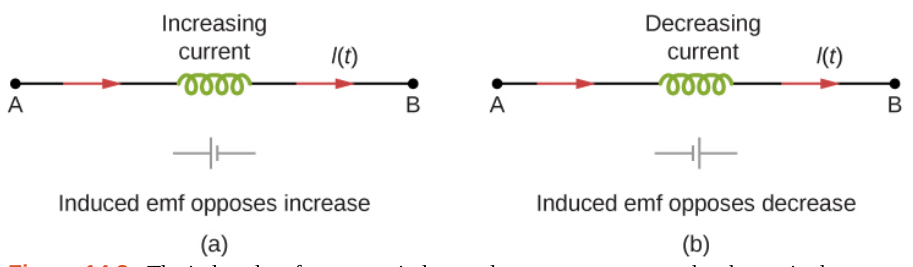
\includegraphics[width=0.9\textwidth,trim=0cm 1.5cm 0cm 0cm,clip=true]{figures/ind4.png}
\caption{\label{fig:ind} (a) Increasing current yields a negative voltage. (b) Decreasing current yields a positive voltage.}
\end{figure}
\end{frame}

\begin{frame}{Inductors}
Suppose we have an inductor with $L = 0.1$ mH, carrying a current of 100 mA.  If we switch off the current in 1 ms, what is the induced emf?
\begin{itemize}
\item A: 0.1 mV
\item B: 1 mV
\item C: 10 mV
\item D: 100 mV
\end{itemize}
\footnotesize
(Ahh, units ... Got heem!  Also, why are the answers \textit{positive?})
\end{frame}

\begin{frame}{Inductors}
Suppose we have a current that switches from 100 mA to -100 mA in 1 ms.  We observe a 100 mV emf across the inductor.  What is the inductance?
\begin{itemize}
\item A: -0.5 mH
\item B: -0.5 H
\item C: 0.5 H 
\item D: 0.5 mH
\end{itemize}
\end{frame}

\begin{frame}{Inductors}
What is the \textbf{\alert{inductance}} of a solenoid, given solenoid properties?  Recall how the inductance relates to flux, current, and turn number:
\begin{align}
L =& N \frac{\Delta \Phi}{\Delta I} \\
L =& N \frac{A \Delta B }{\Delta I} \\
\Delta B =& \mu_0 \left(\frac{N}{l}\right) \Delta I \\
L =& N\frac{A \mu_0 (N/l) \Delta I}{\Delta I} \\
\Aboxed{L =& \frac{\mu_0 N^2 A}{l}} \label{eq:solenoid_ind}
\end{align}
\end{frame}

\begin{frame}{Inductors}
Recall the solenoid used in the Amp\`{e}re's Law lab activity.  Suppose we count $N = 80$ turns, and measure $A = 8 \times 10^{-3}$ m$^2$, and $l = 0.1$ m.  What is the inductance?
\begin{itemize}
\item A: 0.6 H
\item B: 0.06 H
\item C: 6 mH 
\item D: 0.6 mH
\end{itemize}
\footnotesize
Recall that $\mu_0 = 4\pi \times 10^{-7}$ T A$^{-1}$ m.
\end{frame}

\begin{frame}{Inductors}
What is the inductance of the same solenoid, but with twice the turns?
\begin{itemize}
\item A: 2.4 mH
\item B: 1.2 mH
\item C: 24 mH 
\item D: 12 mH
\end{itemize}
\footnotesize
This is a scaling problem.  How does $L$ depend on $N$?
\end{frame}

\begin{frame}{Inductors}
\small
How much \textbf{\alert{energy}} is stored in an inductor?  Suppose potential energy is considered at \textit{a constant voltage}, given some charging circuit that pushes current through an inductor (with some resistance).
\begin{align}
\Delta U &= \Delta q \epsilon ~~ \rightarrow ~~ \epsilon = \Delta U/\Delta q \\
|\epsilon| &= \frac{\Delta U}{\Delta q} = L \frac{\Delta I}{\Delta t} \\
\Delta U &= L \Delta I \left( \frac{\Delta q}{\Delta t} \right) \\
\Delta U &= L I \Delta I \\
\Aboxed{ U &= \frac{1}{2} L I^2}
\end{align}
\footnotesize
\textit{If you do not know how to integrate in the last step, consider the analogy of the area of a triangle.}
\end{frame}

\begin{frame}{Inductors}
How much energy is stored in an inductor with inductance 50 mH that was charged with a current that reaches 1 A?
\begin{itemize}
\item A: 25 J
\item B: 2.5 J
\item C: 25 mJ 
\item D: 2.5 mJ
\end{itemize}
\footnotesize
Nom nom nom, more units.
\end{frame}

\section{A Massive Clue about Electricity and Magnetism}

\begin{frame}{A Massive Clue}
\begin{columns}[T]
\begin{column}{0.5\textwidth}
\footnotesize
The energy stored in a \textbf{\alert{capacitor:}}
\begin{align}
\Delta U &= \Delta q \epsilon ~ \rightarrow ~ \epsilon = \Delta U/\Delta q \\
q &= C \epsilon \\
q &= C \frac{\Delta U}{\Delta q} \\
C^{-1} q \Delta q &= \Delta U \\
\Aboxed{U &= \frac{1}{2}\frac{q^2}{C}}
\end{align}
\end{column}
\begin{column}{0.5\textwidth}
\footnotesize
The energy stored in an \textbf{\alert{inductor:}}
\begin{align}
\Delta U &= \Delta q \epsilon ~ \rightarrow ~ \epsilon = \Delta U/\Delta q \\
|\epsilon| &= \frac{\Delta U}{\Delta q} = L \frac{\Delta I}{\Delta t} \\
\Delta U &= L \Delta I \left( \frac{\Delta q}{\Delta t} \right) \\
\Delta U &= L I \Delta I \\
\Aboxed{ U &= \frac{1}{2} L I^2}
\end{align}
\end{column}
\end{columns}
\footnotesize
It seems the energy stored in a capacitor is \textit{in the E-field}, and the energy stored in the inductor is \textit{in the B-field}.  Suppose we charge a parallel plate capacitor and solenoid ($N = 1$) charged with the same current, $I$, that have the same cross-sectional area $A$, and the same length $d$, such that they have equal energies?
\end{frame}

\begin{frame}{A Massive Clue}
\small
\begin{columns}[T]
\begin{column}{0.5\textwidth}
Assume the proper formulas for capacitance and inductance, and equate energies.
\begin{align}
C =& \frac{\epsilon_0 A}{d} \\
L =& \frac{\mu_0 N^2 A}{d} \\
U_{\rm C} &= U_{\rm L} \\
\frac{1}{2}\frac{Q^2}{C} &= \frac{1}{2}LI^2 \\
\frac{Q^2 d}{\epsilon_0 A} &= \frac{\mu_0 N^2 A I^2}{d} \\
N &= 1 \\
\frac{1}{\epsilon_0 \mu_0} \frac{Q^2}{I^2} &= \frac{A^2}{d^2}
\end{align}
\end{column}
\begin{column}{0.5\textwidth}
Recall that the currents used to charge the capacitor and inductor are the same.
\begin{equation}
\frac{Q^2}{I^2} = t^2
\end{equation}
Note that the volumes of the capacitor and inductor are both $V = Ad$.  Let the lateral dimension of the capacitors (parallel to $A$) be $x$, and 
\begin{equation}
A = \pi x^2
\end{equation}
Combining formulas,
\begin{equation}
\frac{1}{\epsilon_0 \mu_0} = \frac{\pi x^2}{t^2} = v^2
\end{equation}
\end{column}
\end{columns}
\end{frame}

\begin{frame}{A Massive Clue}
\large
The result is a constant \textbf{\alert{velocity!}}  Solving for $v$,
\begin{equation}
\boxed{v = \frac{1}{\sqrt{\epsilon_0 \mu_0}}}
\end{equation}
Insert known values for $\epsilon_0$ and $\mu_0$.  What speed do you obtain?
\begin{itemize}
\item A: $3\times 10^{6}$ m/s
\item B: $3\times 10^{7}$ m/s
\item C: $3\times 10^{8}$ m/s
\item D: $3\times 10^{9}$ m/s
\end{itemize}
\end{frame}

{
\setbeamertemplate{background} 
{
    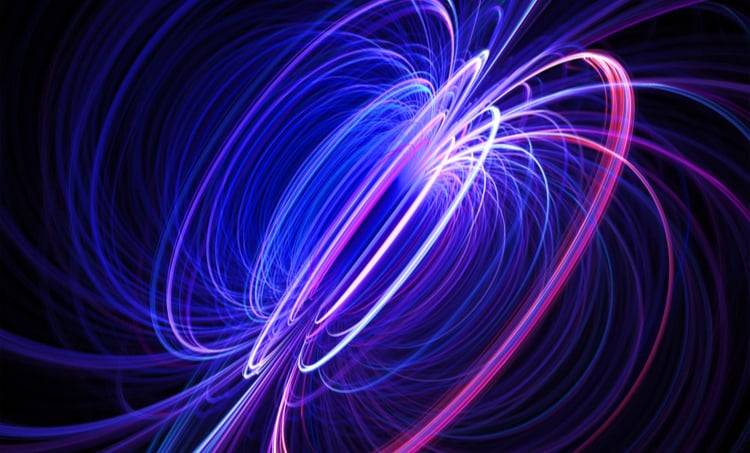
\includegraphics[width=\paperwidth,height=\paperheight]{figures/clue.png}
}
\begin{frame}{The speed of light appears in electromagnetic energy}
\end{frame}
}

\section{RL Circuits}

\begin{frame}{RL Circuits}
An \textbf{\alert{RL circuit}} is a circuit with some resistance $R$ and some inductance $L$.
\begin{figure}
\centering
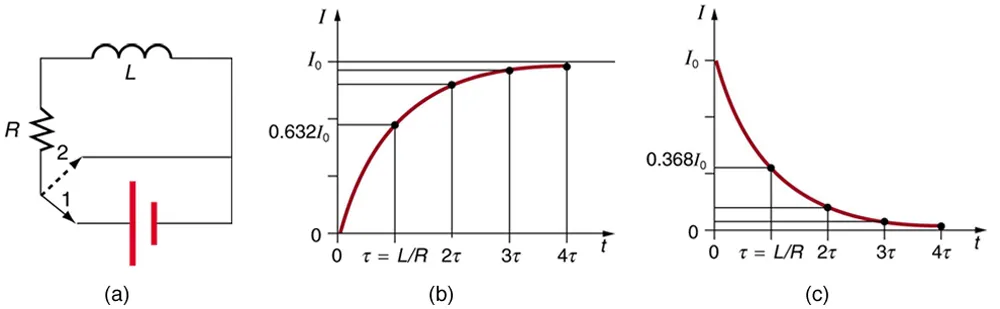
\includegraphics[width=0.9\textwidth]{figures/RL_circuit.png}
\caption{\label{fig:RL} (a) Put switch in lower position to charge inductor, and put switch in upper position to discharge it. (b) The charging current takes a characteristic time to reach the steady state.  (d) The discharging current takes a characteristic time to reach zero.}
\end{figure}
\end{frame}

\begin{frame}{RL Circuits}
\small
Applying Kirchhoff's loop rule to Fig. \ref{fig:RL} (a), we have
\begin{equation}
\mathcal{E} - iR - L \frac{\Delta I}{\Delta t} = 0
\end{equation}
\footnotesize
\begin{itemize}
\item $\mathcal{E}$ is a positve emf in the loop direction.
\item The second term is negative because the resistor \textit{decreases the voltage} by consuming energy.  The side with the larger voltage is towards the emf.
\item The third term is negative because the inductor \textit{produces an emf} counteracting the positive emf.  The side with the larger voltage is towards the emf.
\item There is an exact solution to this equation.  Let $\tau = L/R$:
\begin{equation}
i(t) = \frac{\mathcal{E}}{R}\left(1 - e^{-tR/L}\right)
\end{equation}
\end{itemize}
\end{frame}

\begin{frame}{RL Circuits}
Letting $i_0 = \mathcal{E}/R$, and $\tau = L/R$,
\begin{equation}
i(t) = i_0\left(1 - e^{-t/\tau}\right)
\end{equation}
Suppose an RL circuit has an inductance of 1 mH and a resistance of 1 k$\Omega$.  What is the time constant?
\begin{itemize}
\item A: 1 millisecond
\item B: 1 microsecond
\item C: 1 nanosecond
\item D: 1 second
\end{itemize}
\end{frame}

\begin{frame}{RL Circuits}
Letting $i_0 = \mathcal{E}/R$, and $\tau = L/R$,
\begin{equation}
i(t) = i_0\left(1 - e^{-t/\tau}\right)
\end{equation}
If $\tau = 1 \mu$s, and $R = 1$ k$\Omega$, with $\mathcal{E} = 5$V, what will the current be after 100 $\mu$s?
\begin{itemize}
\item A: 1 mA
\item B: 5 A
\item C: 5 mA
\item D: 1 A
\end{itemize}
\end{frame}

\begin{frame}{RL Circuits}
Letting $i_0 = \mathcal{E}/R$, and $\tau = L/R$,
\begin{equation}
i(t) = i_0\left(1 - e^{-t/\tau}\right)
\end{equation}
If $\tau = 1 \mu$s, and $R = 1$ k$\Omega$, with $\mathcal{E} = 5$V, what will the current be at 1 $\mu$s?
\begin{itemize}
\item A: 1.20 mA
\item B: 3.16 mA
\item C: 4.12 mA
\item D: 10.1 mA
\end{itemize}
\end{frame}

\begin{frame}{RL Circuits}
\footnotesize
\begin{figure}
\centering
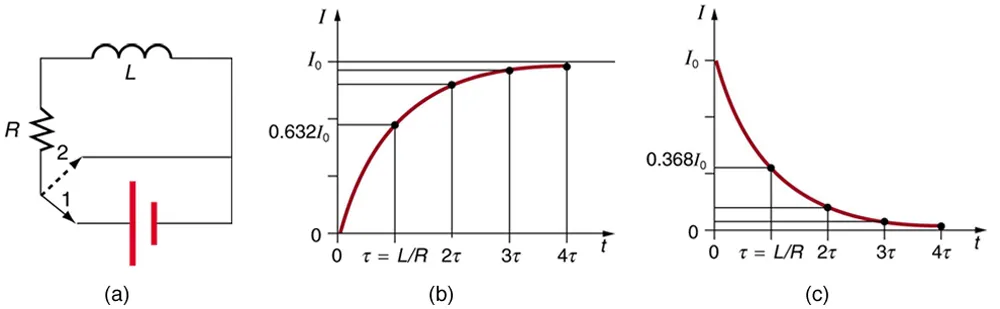
\includegraphics[width=0.7\textwidth]{figures/RL_circuit.png}
\caption{\label{fig:RL2} Current discharge is not instantaneous (c).}
\end{figure}
Inductor discharge in RL circuit:
\begin{equation}
i(t) = i_0 e^{-t/\tau}
\end{equation}
What is the current as $t \to \infty$?  What is the current at $t=0$?
\begin{itemize}
\item A: 0, $R/\mathcal{E}$
\item B: 0, $\mathcal{E}/R$
\item C: $\mathcal{E}/R$
\item D: $R/\mathcal{E}$, 0
\end{itemize}
\end{frame}

\section{RL Circuits Application: Signal Filters and PhET}

\begin{frame}{PhET: RL and RC Circuits as Filters}
\small
RC and RL circuits can act as \textit{high-pass} and \textit{low-pass} \textbf{\alert{signal filters.}}
\begin{itemize}
\item In the \textbf{\alert{RC circuit}}, with $\tau = RC$, the capacitor \textit{voltage} charges and discharges like
\begin{align}
V_{charge}(t) &= V_0 \left(1 - e^{-t/\tau}\right) \\
V_{discharge}(t) &= V_0 e^{-t/\tau}
\end{align}
\item In the \textbf{\alert{RL circuit}}, with $\tau = L/R$, the inductor \textit{current} charges and discharges like
\begin{align}
i_{charge}(t) &= i_0 \left(1 - e^{-t/\tau}\right) \\
i_{discharge}(t) &= i_0 e^{-t/\tau}
\end{align}
\end{itemize}
\end{frame}

\begin{frame}{PhET: RL and RC Circuits as Filters}
\footnotesize
Go to \url{https://phet.colorado.edu/en/simulations/circuit-construction-kit-ac}.
\begin{itemize}
\footnotesize
\item In the AC Circuits PhET simulator, create an \textbf{\alert{RC circuit}}, with $R = 8 \Omega$, and $C = 0.05$ F (50 mF), and a AC voltage source set to 120V amplitude.
\begin{enumerate}
\footnotesize
\item Click and drag a voltage chart from the right side to measure the AC source voltage.
\item Click and drag a voltage chart from the right side to measure the capacitor voltage.
\item Create a spreadsheet with three columns: (1) frequency of the AC voltage source, (2) peak AC voltage source amplitude, and (3) peak capacitor voltage amplitude.
\end{enumerate}
\end{itemize}
\end{frame}

\begin{frame}{PhET: RL and RC Circuits as Filters}
\footnotesize
Go to \url{https://phet.colorado.edu/en/simulations/circuit-construction-kit-ac}.
\begin{itemize}
\footnotesize
\item In the AC Circuits PhET simulator, create an \textbf{\alert{RL circuit}}, with $R = 10 \Omega$, and $L = 1.0$ H, and a AC voltage source set to 120V amplitude.
\begin{enumerate}
\footnotesize
\item Click and drag a voltage chart from the right side to measure the AC source voltage.
\item Click and drag a voltage chart from the right side to measure the inductor voltage.
\item Create a spreadsheet with three columns: (1) frequency of the AC voltage source, (2) peak AC voltage source amplitude, and (3) peak capacitor voltage amplitude.
\end{enumerate}
\end{itemize}
\end{frame}

\begin{frame}{PhET: RL and RC Circuits as Filters}
\footnotesize
\begin{enumerate}
\item Create a graph with a range [0.0,1.0] for the y-axis, for a unitless ratio, and a domain of [0.0,2.0] Hz for the x-axis.
\item Plot the ratio of $V_{\rm C}/V_{\rm source}$ versus frequency on your graph.
\item Plot the ratio of $V_{\rm L}/V_{\rm source}$ versus frequency on your graph.
\item For a \textbf{bonus point}, convert your ratio to decibels (dB, $20\log_{10}(ratio)$).
\item Which AC circuit is the \textit{low-pass} filter, and which AC circuit is the \textit{high-pass} filter?  How is energy conserved if the voltage changes?
\end{enumerate}
\begin{figure}
\centering
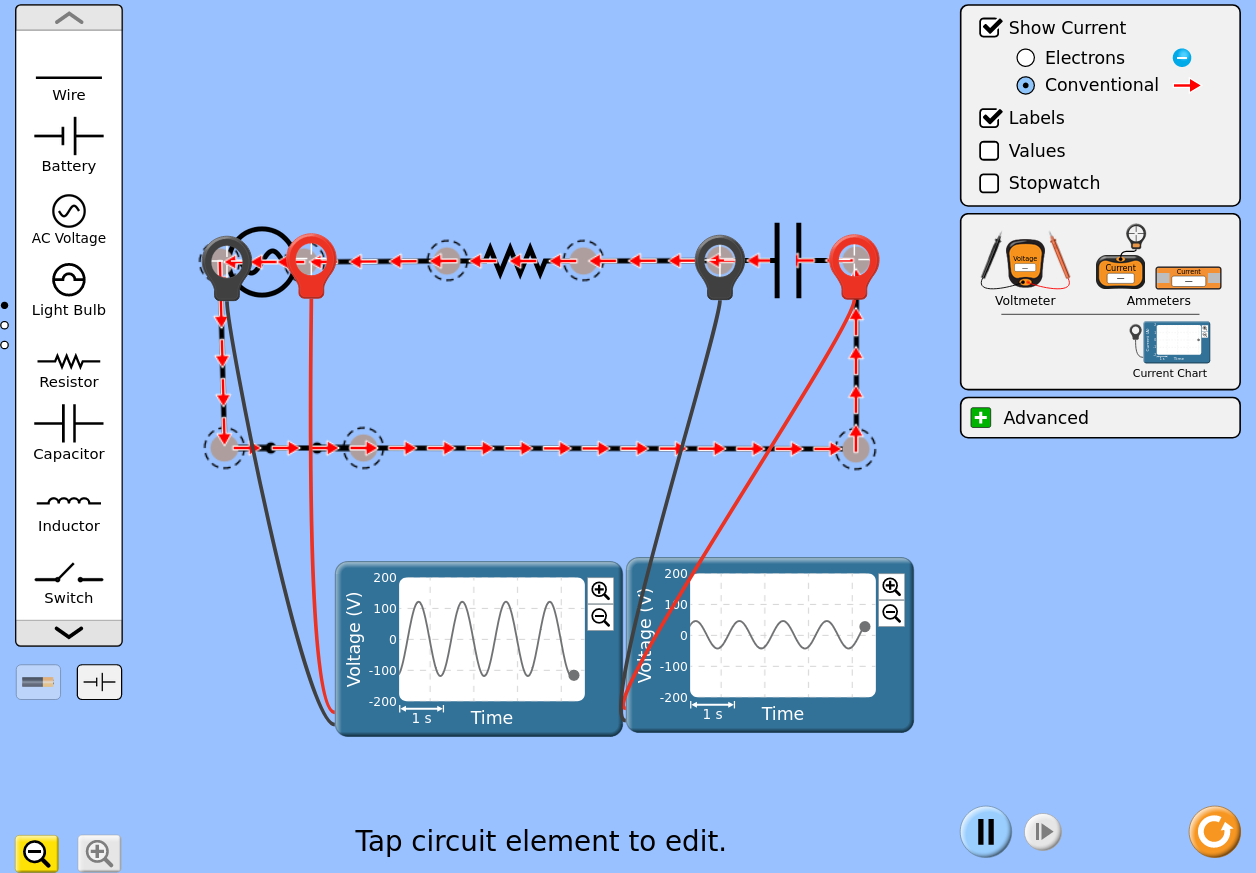
\includegraphics[width=0.35\textwidth]{figures/RC_PhET.png}
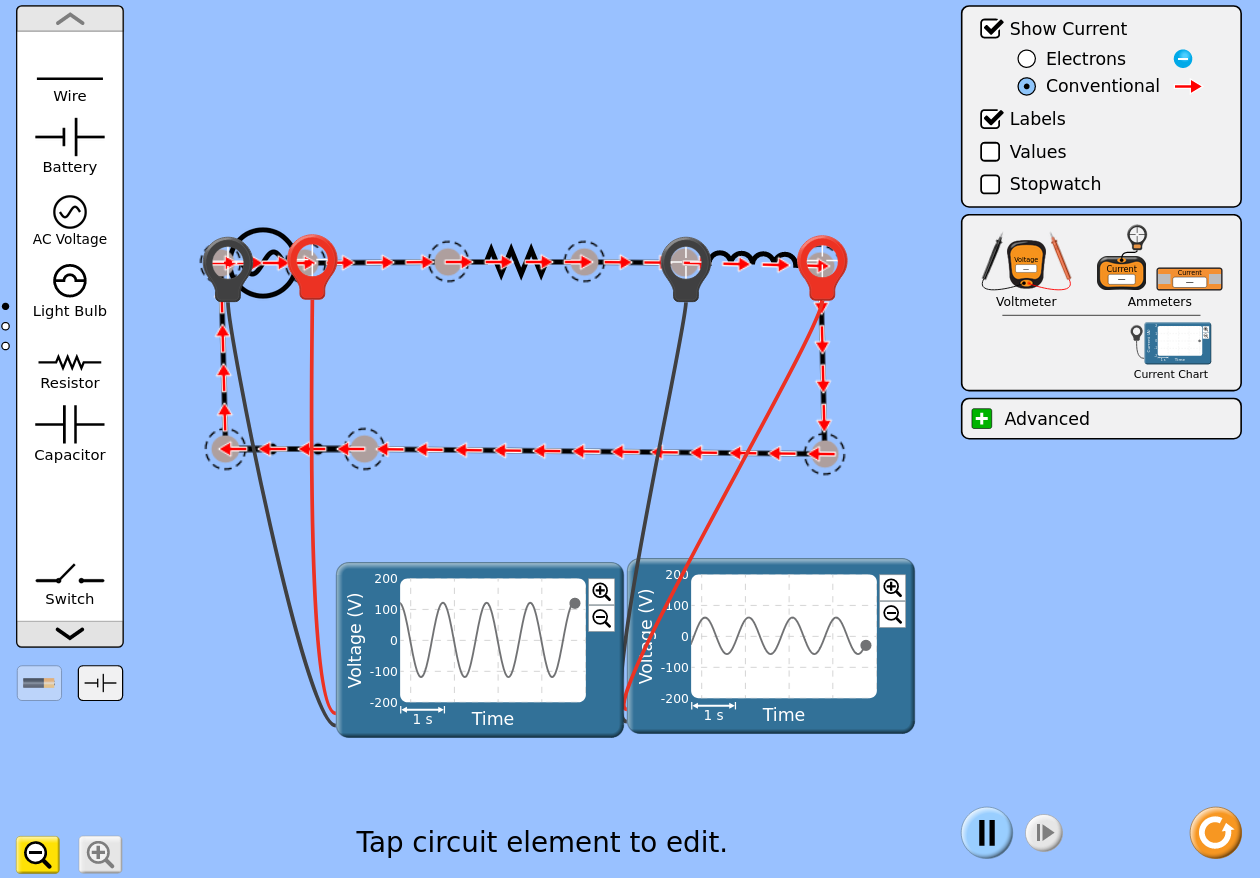
\includegraphics[width=0.35\textwidth]{figures/RL_PhET.png}
\caption{\label{fig:RC_RL_PhET} \footnotesize (Left) Example of the RC circuit. (Right) Example of the RL circuit.}
\end{figure}
\end{frame}

\section{Reactance, Inductive and Capacitive}

\begin{frame}{Reactance, Inductive and Capacitive}
\small
\textbf{\alert{Reactance}} is resistance that is associated with a change in the signal \textit{phase.}  What is the phase?
\begin{figure}
\centering
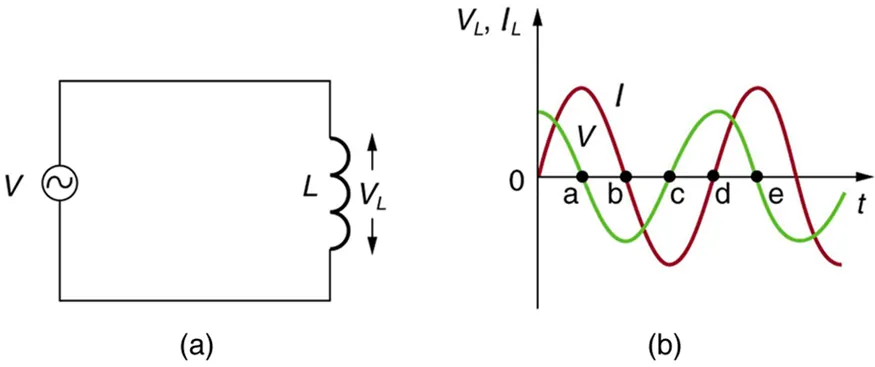
\includegraphics[width=0.85\textwidth]{figures/phase.png}
\caption{\label{fig:phase} (a) An AC source connected to an inductor. (b) Voltage and current at the inductor are no longer \textit{in-phase.}  Voltage leads the current by a 90 degree phase shift.}
\end{figure}
\end{frame}

\begin{frame}{Reactance, Inductive and Capacitive}
\begin{tcolorbox}[colback=white,colframe=black!40!black,title=Phase Shift of a Sinusoid]
\alert{Let a time-dependent signal have an amplitude $A$, frequency $f$, and phase $\phi$:
\begin{equation}
s(t) = A\cos(2\pi f t + \phi)
\end{equation}
Two signals with phases $\phi_1$ and $\phi_2$ have a relative \textit{phase shift} $\Delta \phi = \phi_2 - \phi_1$, measured in degrees or radians.}
\end{tcolorbox}
\end{frame}

\begin{frame}{Reactance, Inductive and Capacitive}
\begin{figure}
\centering
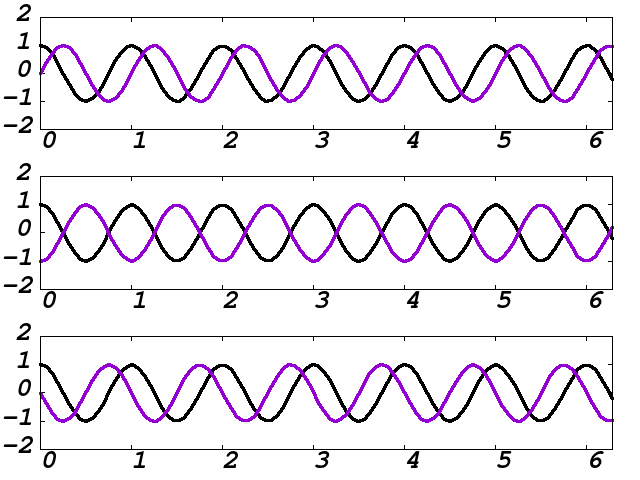
\includegraphics[width=0.75\textwidth]{figures/phase2.png}
\caption{\label{fig:phase2} (Top) $\Delta\phi = 90$ deg. (Middle) $\Delta\phi = 180$ deg. (Bottom) $\Delta\phi = 270$ deg.}
\end{figure}
\end{frame}

\begin{frame}{Reactance, Inductive and Capacitive}
\begin{tcolorbox}[colback=white,colframe=black!40!black,title=Reactance and Inductors]
\alert{Let $\phi_{\rm V}$ and $\phi_{\rm I}$ be the phase of the voltage and current.  When a sinusoidal voltage is applied to an inductor:
\begin{equation}
\phi_{\rm V} - \phi_{\rm I} = \pi/2
\end{equation}
The voltage leads the current by a 90 degree phase shift.  The reactance from the inductor is $X_{\rm L}$, and fits into Ohm's law like $V = I X_{\rm L}$, where $V$ and $I$ are the rms voltage and current.  Finally,
\begin{equation}
X_{\rm L} = 2\pi f L
\end{equation}
\footnotesize
Units: 1 H is $1 \Omega$ s, and frequency is 1 Hz, or 1 s$^{-1}$.}
\end{tcolorbox}
\end{frame}

\begin{frame}{Reactance, Inductive and Capacitive}
Suppose the reactance of an inductor is $1$ k$\Omega$ at a frequency of 1 kHz.  What is the inductance?
\begin{itemize}
\item A: $2\pi$ Henries
\item B: $2\pi$ Ohms
\item C: $1/(2\pi)$ Henries
\item D: $1/(2\pi$ Ohms
\end{itemize}
\end{frame}

\begin{frame}{Reactance, Inductive and Capacitive}
What is the reactance at half the frequency, 0.5 kHz?
\begin{itemize}
\item A: $\pi$ Henries
\item B: $\pi$ Ohms
\item C: $1/(4\pi)$ Henries
\item D: $1/(4\pi$ Ohms
\end{itemize}
\footnotesize
Hint, treat this like a scaling problem.
\end{frame}

\begin{frame}{Reactance, Inductive and Capacitive}
Suppose we are dealing with a \textit{series} RL circuit.  The resistor has $R = 1$ k$\Omega$, and the frequency is $1/(2\pi)$ MHz.  If the inductance is 1 mH, what is the total resistance, in k$\Omega$?
\begin{itemize}
\item A: 2 k$\Omega$
\item B: 4 k$\Omega$
\item C: $1/(2\pi)$ k$\Omega$
\item D: $1/(4\pi)$ k$\Omega$
\end{itemize}
\footnotesize
Hint, deal with the units via powers of ten.
\end{frame}

\begin{frame}{Reactance, Inductive and Capacitive}
Suppose we are dealing with the same resistance and inductance, but they are connected \textit{in parallel.}  What is the total resistance?
\begin{itemize}
\item A: 0.25 k$\Omega$
\item B: 1 k$\Omega$
\item C: 0.1 k$\Omega$
\item D: 0.5 k$\Omega$
\end{itemize}
\footnotesize
Recall that series resistances (and reactances) sum differently when they are connected in parallel.
\end{frame}

\begin{frame}{Reactance, Inductive and Capacitive}
What is the rms current in a series RL circuit with $R = 1$ k$\Omega$, and $X_{\rm L} = 1$ k$\Omega$, if the rms voltage is 120 V?
\begin{itemize}
\item A: 60 A
\item B: 120 mA
\item C: 60 mA
\item D: 120 mA
\end{itemize}
\end{frame}

\begin{frame}{Reactance, Inductive and Capacitive}
\small
\textbf{\alert{Reactance}} is resistance that is associated with a change in the signal \textit{phase.}  What is the phase?
\begin{figure}
\centering
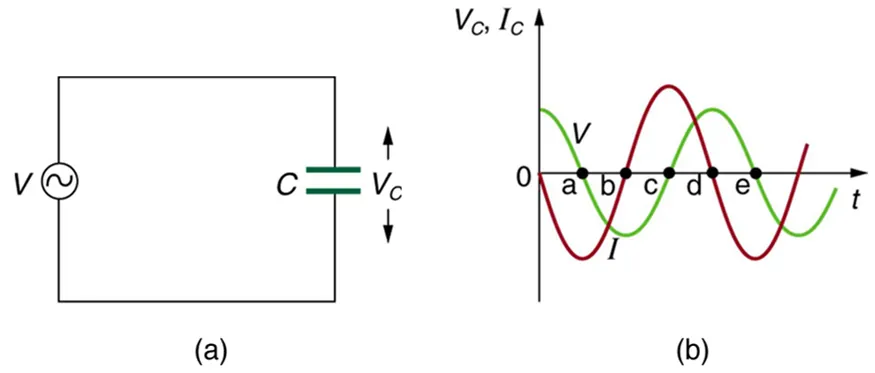
\includegraphics[width=0.85\textwidth]{figures/phase3.png}
\caption{\label{fig:phase3} (a) An AC source connected to a capacitor. (b) Voltage and current at the inductor are no longer \textit{in-phase.}  Current leads the voltage by a 90 degree phase shift.}
\end{figure}
\end{frame}

\begin{frame}{Reactance, Inductive and Capacitive}
\begin{tcolorbox}[colback=white,colframe=black!40!black,title=Reactance and Capacitors]
\alert{Let $\phi_{\rm V}$ and $\phi_{\rm I}$ be the phase of the voltage and current.  When a sinusoidal voltage is applied to a capacitor:
\begin{equation}
\phi_{\rm V} - \phi_{\rm I} = -\pi/2
\end{equation}
The voltage lags the current by a 90 degree phase shift.  The reactance from the capacitor is $X_{\rm C}$, and fits into Ohm's law like $V = I X_{\rm C}$, where $V$ and $I$ are the rms voltage and current.  Finally,
\begin{equation}
X_{\rm C} = \frac{1}{2\pi f C}
\end{equation}
\footnotesize
Units: 1 F = C V$^{-1}$, $f \rightarrow 1$ s$^{-1}$, and 1 A V$^{-1}$ is $\Omega^{-1}$, $X_{\rm C} \rightarrow 1/(1/\Omega) = \Omega$.}
\end{tcolorbox}
\end{frame}

\begin{frame}{Reactance, Inductive and Capacitive}
Suppose the reactance of a capacitor is $1$ k$\Omega$ at a frequency of 1 kHz.  What is the capacitance?
\begin{itemize}
\item A: $2\pi$ $\mu$F
\item B: $2\pi$ F
\item C: $1/(2\pi)$ $\mu$F
\item D: $1/(2\pi$ F
\end{itemize}
\end{frame}

\begin{frame}{Reactance, Inductive and Capacitive}
What is the reactance at half the frequency, 0.5 kHz?
\begin{itemize}
\item A: $\pi$ F
\item B: $\pi$ $\mu$F
\item C: $1/(\pi)$ $\mu$F
\item D: $1/(\pi)$ F
\end{itemize}
\footnotesize
Hint, treat this like a scaling problem.
\end{frame}

\begin{frame}{Reactance, Inductive and Capacitive}
Suppose we are dealing with a \textit{series} RC circuit.  The resistor has $R = 1$ k$\Omega$, and the frequency is $1/(2\pi)$ kHz.  If the capacitance is 1 $\mu$F, what is the total resistance, in k$\Omega$?
\begin{itemize}
\item A: $1/(4\pi)$ k$\Omega$
\item B: 4 k$\Omega$
\item C: $1/(2\pi)$ k$\Omega$
\item D: 2 k$\Omega$
\end{itemize}
\footnotesize
Hint, deal with the units via powers of ten.
\end{frame}

\begin{frame}{Reactance, Inductive and Capacitive}
Suppose we are dealing with the same resistance and inductance, but they are connected \textit{in parallel.}  What is the total resistance?
\begin{itemize}
\item A: 0.25 k$\Omega$
\item B: 1 k$\Omega$
\item C: 0.1 k$\Omega$
\item D: 0.5 k$\Omega$
\end{itemize}
\footnotesize
Recall that series resistances (and reactances) sum differently when they are connected in parallel.
\end{frame}

\begin{frame}{Reactance, Inductive and Capacitive}
What is the rms current in a series RC circuit with $R = 1$ k$\Omega$, and $X_{\rm C} = 1$ k$\Omega$, if the rms voltage is 120 V?
\begin{itemize}
\item A: 60 mA
\item B: 120 mA
\item C: 60 A
\item D: 120 mA
\end{itemize}
\end{frame}

\begin{frame}{Reactance, Inductive and Capacitive}
\small
\textbf{\alert{Reactance}} is resistance that is associated with a change in the signal \textit{phase.}  What is the phase?
\begin{figure}
\centering
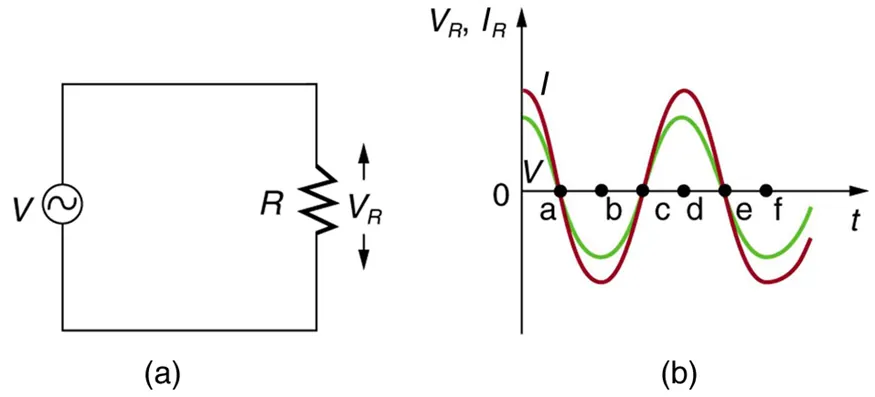
\includegraphics[width=0.85\textwidth]{figures/phase4.png}
\caption{\label{fig:phase4} (a) An AC source connected to a resistor. (b) Voltage and current at the inductor are \textit{in-phase.}  Current and voltage have a phase shift of 0 degrees.}
\end{figure}
\end{frame}

\section{RLC Circuits}

\begin{frame}{RLC Circuits}
\small
A generalization of \textbf{\alert{Ohm's Law}} for AC circuits that involve resistance, capacitance, and inductance is
\begin{align}
V_{\rm rms} &= I_{\rm rms} Z \\
V_{0} &= I_{0} Z
\end{align}
The \textbf{\alert{impedance}} is $Z$, and subscripts refer to the rms and peak values.
\begin{figure}
\centering
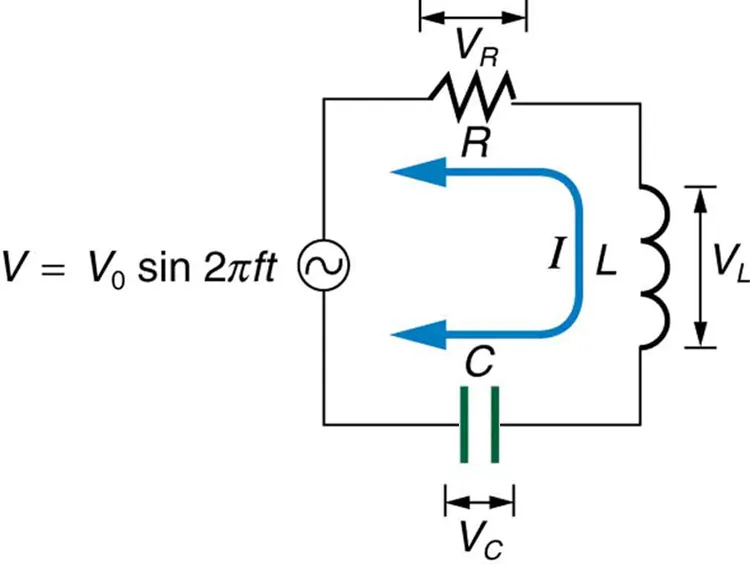
\includegraphics[width=0.45\textwidth]{figures/phase5.png}
\caption{\label{fig:phase5} An AC source connected to an RLC circuit.}
\end{figure}
\end{frame}

\begin{frame}{RLC Circuits}
\small
A generalization of \textbf{\alert{Ohm's Law}} for AC circuits that involve resistance, capacitance, and inductance is
\begin{align}
V_{\rm rms} &= I_{\rm rms} Z \\
V_{0} &= I_{0} Z
\end{align}
The \textbf{\alert{impedance}} is $Z$, and subscripts refer to the rms and peak values.
\begin{figure}
\centering
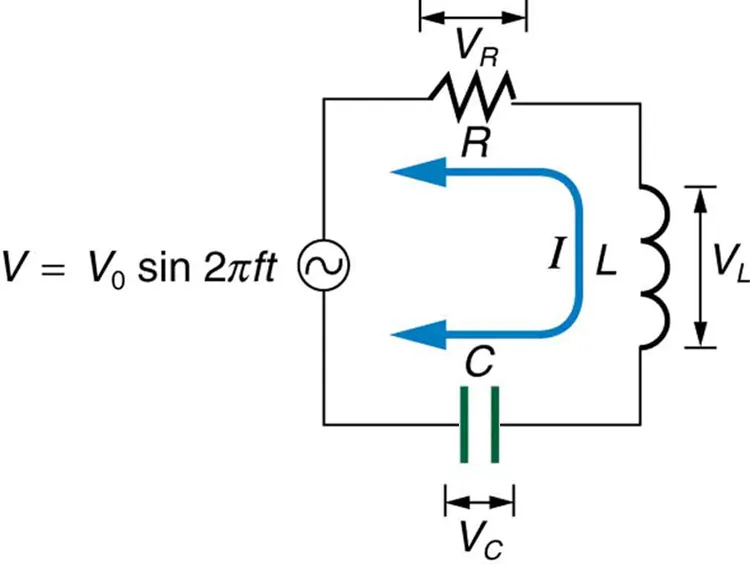
\includegraphics[width=0.45\textwidth]{figures/phase5.png}
\caption{\label{fig:phase6} An AC source connected to an RLC circuit.}
\end{figure}
\end{frame}

\begin{frame}{RLC Circuits}
\footnotesize
\begin{figure}
\centering
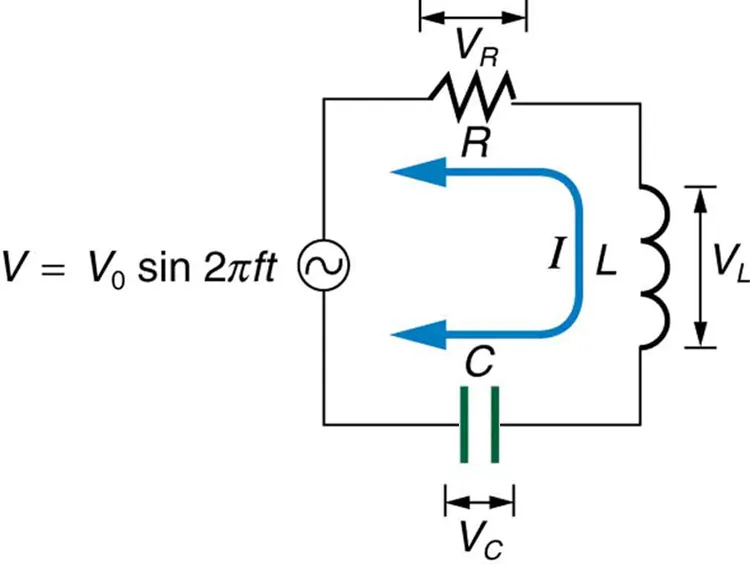
\includegraphics[width=0.33\textwidth]{figures/phase5.png}
\caption{\label{fig:phase7} How do we calculate impedance in the RLC circuit, and how do we predict the behavior of current?}
\end{figure}
We cannot simply \textbf{\alert{sum}} the impedances of the R, L, and C components.  The reason is \textit{phase}:
\begin{align}
\phi_{\rm V,RL} - \phi_{\rm I,RL} &= \pi/2 \\
\phi_{\rm V,RC} - \phi_{\rm I,RC} &= -\pi/2 \\
\phi_{\rm V,RLC} - \phi_{\rm I,RLC} &= \pi
\end{align}
The phase shift between the inductor and capacitor voltages is 180 degrees.
\end{frame}

\begin{frame}{RLC Circuits}
\begin{figure}
\centering
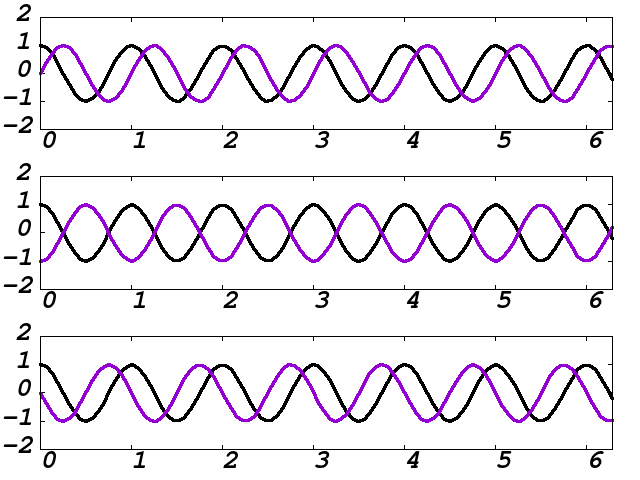
\includegraphics[width=0.85\textwidth,trim=1cm 5cm 0cm 4cm,clip=true]{figures/phase2.png}
\caption{\label{fig:phase8} Two sinusoids with a relative phase shift of 180 degrees.}
\end{figure}
Using complex numbers to represent $Z_{\rm R}$, $Z_{\rm L}$, and $Z_{\rm C}$, we can show that the \textbf{\alert{total impedance}} follows
\begin{equation}
Z = \sqrt{R^2 + \left(X_{\rm L} - X_{\rm C} \right)^2}
\end{equation}
\end{frame}

\begin{frame}{RLC Circuits}
An RLC circuit is set up at $f = 10$ kHz with $R = 1$ k$\Omega$, $X_{\rm L} = 0.5$ k$\Omega$ and $X_{\rm C} = 2$ k$\Omega$, what is the total $Z$?
\begin{itemize}
\item A: 1.0 k$\Omega$
\item B: 1.8 k$\Omega$
\item C: 0.9 k$\Omega$
\item D: 2.0 k$\Omega$
\end{itemize}
\end{frame}

\begin{frame}{RLC Circuits}
What is the total $Z$ if the frequency is \textit{doubled} to 20 kHz?
\begin{itemize}
\item A: 1.0 k$\Omega$
\item B: 1.8 k$\Omega$
\item C: 0.9 k$\Omega$
\item D: 2.0 k$\Omega$
\end{itemize}
What do you notice about this impedance?
\begin{itemize}
\item A: It is the minimum total impedance.
\item B: It is the maximum total impedance.
\item C: $Z = R$
\item D: A and C
\end{itemize}
\end{frame}

\begin{frame}{RLC Circuits}
\small
Consider \textbf{\alert{Ohm's law}}, and the RLC \textbf{\alert{impedance}}:
\begin{equation}
I_{\rm rms} = \frac{V_{\rm rms}}{\sqrt{R^2 + \left(X_{\rm L} - X_{\rm C} \right)^2}}
\end{equation}
Setting $X_{\rm L} = X_{\rm C}$, we find the original form of Ohm's Law for AC circuits: $I_{\rm rms} = V_{\rm rms}/R$.  Because $\left(X_{\rm L} - X_{\rm C} \right)^2$ is always positive, current is maximized when the inductor and capacitor reactance are equal.  This implies
\begin{align}
X_{\rm L} &= X_{\rm C} \\
2\pi f L &= \frac{1}{2\pi f C} \\
\Aboxed{f &= \frac{1}{2\pi\sqrt{LC}}}
\end{align}
Given $L$ and $C$, there is a \textit{resonance frequency} that maximizes current.
\end{frame}

\begin{frame}{RLC Circuits}
\begin{columns}[T]
\begin{column}{0.5\textwidth}
The resonance frequency is
\begin{equation}
f = \frac{1}{2\pi\sqrt{LC}}
\end{equation}
\begin{figure}
\centering
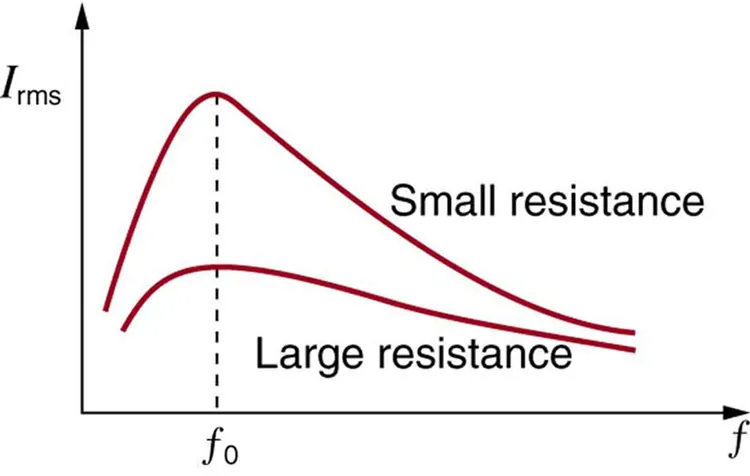
\includegraphics[width=0.95\textwidth]{figures/resonance.png}
\caption{\label{fig:resonance} The peak and width of $I_{\rm rms}$ vs. $f$ is controlled by choices for R, L, and C.}
\end{figure}
\end{column}
\begin{column}{0.5\textwidth}
What is the resonance frequency for an RLC circuit with $L = 1$ $\mu$H and $C = 1$ $\mu$F?
\begin{itemize}
\item A: $1/(2\pi)$ Hz
\item B: $1$ kHz
\item C: $1/(2\pi)$ GHz
\item D: $1/(2\pi)$ MHz
\end{itemize}
\end{column}
\end{columns}
\end{frame}

\begin{frame}{RLC Circuits}
also decide how to cover ``power factor'' $P = I V \cos\theta$
\end{frame}

\section{PhET: RLC Circuits and Resonance}

\section{Conclusion}

\begin{frame}{Summary}
\begin{enumerate}
\item Magnetic induction - \textbf{Chapters 23.1 - 23.5, 23.7, 23.9}
\begin{itemize}
\item Induced EMF and magnetic flux
\item Faraday's Law
\item Motional EMF, generators, and transformers
\end{itemize}
\item AC circuits - \textbf{Chapters 23.9 - 23.12}
\begin{itemize}
\item Inductors
\item RL circuits
\item RLC circuits
\end{itemize}
\end{enumerate}
\end{frame}

\end{document}
